% \subsection{Physical limits}
% \label{sec:physical limits}

One of the promising and simple ways to set and enforce limit on the number of forwarded Interests is a variation of the well-known bag of tokens algorithm, illustrated on Fig.~\ref{fig:bag of tokens}.
Each router implementing the algorithm maintains a ``bag'' with a limited number of tokens for every outgoing interface.
Whenever an Interest is ready to be forwarded, the router ``borrows'' a token from the outgoing interface's bag, dropping the Interest if the bag is empty.
At the same time, when the requested Data comes back or the Interest times out, the token is returned to the appropriate bag based on the information in PIT, ready to be borrowed again by a new incoming Interset.

\begin{figure}[htbp]
  \centering
  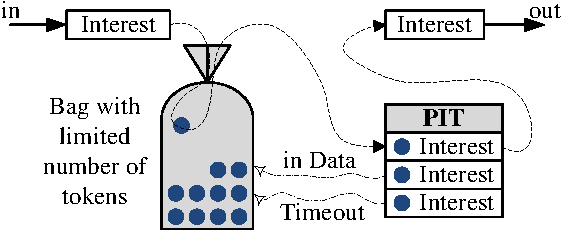
\includegraphics[scale=0.6]{token-bag}
  \caption{Bag of tokens algorithm: tokens borrowed when Interest is forwarded and returned when Data comes back or Interest times out}
  \label{fig:bag of tokens}
\end{figure}

Since the number of tokens in the bag defines how many Interests are forwarded and not yet satisfied or timed out (pending Interests), this number should be large enough to fully utilize the network and small enough to avoid excessive buffering and drops at the upstream routers.
The ideal value for the number of tokens (\emph{Interest Limit}) for each individual link would be defined proportional to the link's bandwidth-delay product (BDP)~\cite{tcp-survey}.
This can be formalized in the following way:
% With the objective to request as many Data packets, as downstream link can pump through, we are getting the following equation for Interest limit:

\begin{equation}
\mathrm{Interest\ Limit} = Delay\ [s] \cdot \frac{\mathrm{Bandwidth\ [Bytes/s]}}{\mathrm{Data\ packet\ size\ [Bytes]}}
\end{equation}

In this equation, \emph{Delay} is the expected time of Interest being satisfied and \emph{Data packet size} is the size of the returned Data packet.
Although both these values are not known a priory and vary between different Interest-Data exchanges, it is not really necessary to know their exact values.
One can simply set the Interest limit based on the average values of round trip time and observed Data packet size, as the network buffers can smooth out most of the network fluctuations.

In the rest of the paper we will refer to Interest limits set based on the bandwidth-delay product as \emph{Physical limits}, as we set the limit based on the physical link capacity.
Pseudocode~\ref{alg:simple limits} shows implementation details of the Physical limits algorithms.
Every time an Interest is ready to be send to an outgoing interface $of$ (\emph{OutInterest} function), we check if the token bag is not empty.
If there is at least one free token available, we are ``borrowing'' it, forwarding the Interests, and remembering the outgoing interface in the corresponding entry of PIT.
Functions \emph{InData} and \emph{Timeout} ensure that tokens are ``returned'' whenever the requested Data is received or Interest times out.

\floatname{algorithm}{Pseudocode}

\begin{algorithm}[h]
\caption{Physical limits}
\label{alg:simple limits}
\begin{algorithmic}[1]
\For{\textbf{each} interface \em{f}}
    \State{$L_{f} \leftarrow$ Interest Limit according to (1)}
    \State{$O_{f} \leftarrow 0$} \Comment{Outstanding Interests on interface \textbf{f}}
\EndFor

\vspace{0.2cm}
\Function{OutInterest}{Interest \textbf{i}, OutInterface \textbf{of}}
    \If{$L_{of} - O_{of} > 0$} \Comment{\textbf{of} is under physical limits}
        \State $O_{of} \leftarrow O_{of} + 1$  \Comment{``Borrow'' token}
        \State add \textbf{of} to PIT entry and forward \textbf{i} to \textbf{of}
    \Else
        \State drop Interest
    \EndIf
\EndFunction

\vspace{0.2cm}

\Function{InData}{Data \textbf{d}}
   \State lookup PIT entry \textbf{p} for data \textbf{d}
   \For{\textbf{each} outgoing interface \textbf{of} in \textbf{p}}
        \State $O_{of} \leftarrow O_{of} - 1$ \Comment{``Return'' token}
   \EndFor
\EndFunction

\vspace{0.2cm}

\Function{Timeout}{PIT entry $i$}
   \For{\textbf{each} outgoing interface \textbf{of} in \textbf{p}}
        \State $O_{of} \leftarrow O_{of} - 1$ \Comment{``Return'' token}
   \EndFor
\EndFunction

\end{algorithmic}
\end{algorithm}


% In our experiments Interest/Data size ratio is about 1:30
Considering the fact that normally the size of the Interests packets is significantly smaller than the size of the requested Data packets, a router needs to consume only a small portion of the upstream link (from A to B) to fully utilize the downstream link (from B to A).
The direct conclusion from this observation, confirmed by our evaluations in the Section~\ref{sec:evaluation}, is that if a router forwards only the right amount of Interests, both mechanisms of the Interests flooding attack will stop working: the forwarded Interests would neither congest the upstream nor exhaust router's memory resources.
At the same time, the Physical limits may become a new mechanisms to carry out denial of service attacks.
For example, if the router A has forwarded 125 junk Interests, it will not be able to accept any other Interests neither from a legitimate user or an adversary, until these junk Interests start to expire.
This essentially reduces the probability of legitimate Interests getting through and can result in an effective low-rate denial of service attack (refer to Section~\ref{sec:small-scale}).


%%% Local Variables: 
%%% mode: latex
%%% TeX-master: "../paper"
%%% End: 
